% Generated file: per-epoch training curves (pure TikZ, values from training logs)
\begin{subfigure}[b]{0.49\textwidth}\centering
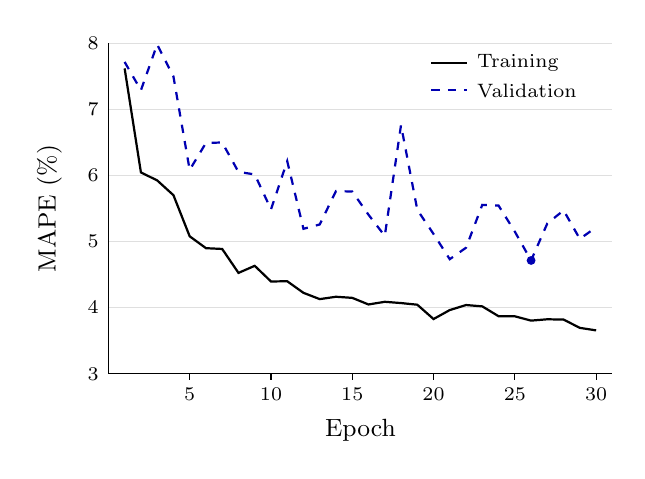
\begin{tikzpicture}[font=\small]
\draw[gray!25] (0,0.000) -- (6.400,0.000);
\node[left,font=\scriptsize] at (0,0.000) {3};
\draw[gray!25] (0,0.840) -- (6.400,0.840);
\node[left,font=\scriptsize] at (0,0.840) {4};
\draw[gray!25] (0,1.680) -- (6.400,1.680);
\node[left,font=\scriptsize] at (0,1.680) {5};
\draw[gray!25] (0,2.520) -- (6.400,2.520);
\node[left,font=\scriptsize] at (0,2.520) {6};
\draw[gray!25] (0,3.360) -- (6.400,3.360);
\node[left,font=\scriptsize] at (0,3.360) {7};
\draw[gray!25] (0,4.200) -- (6.400,4.200);
\node[left,font=\scriptsize] at (0,4.200) {8};
\draw (1.032,0) -- (1.032,-0.08);
\node[below,font=\scriptsize] at (1.032,-0.05) {5};
\draw (2.065,0) -- (2.065,-0.08);
\node[below,font=\scriptsize] at (2.065,-0.05) {10};
\draw (3.097,0) -- (3.097,-0.08);
\node[below,font=\scriptsize] at (3.097,-0.05) {15};
\draw (4.129,0) -- (4.129,-0.08);
\node[below,font=\scriptsize] at (4.129,-0.05) {20};
\draw (5.161,0) -- (5.161,-0.08);
\node[below,font=\scriptsize] at (5.161,-0.05) {25};
\draw (6.194,0) -- (6.194,-0.08);
\node[below,font=\scriptsize] at (6.194,-0.05) {30};
\draw (0,0) -- (6.400,0); \draw (0,0) -- (0,4.200);
\draw[thick, black] (0.206,3.879) -- (0.413,2.558) -- (0.619,2.457) -- (0.826,2.269) -- (1.032,1.747) -- (1.239,1.596) -- (1.445,1.586) -- (1.652,1.282) -- (1.858,1.372) -- (2.065,1.173) -- (2.271,1.176) -- (2.477,1.029) -- (2.684,0.949) -- (2.890,0.979) -- (3.097,0.965) -- (3.303,0.881) -- (3.510,0.915) -- (3.716,0.899) -- (3.923,0.878) -- (4.129,0.696) -- (4.335,0.810) -- (4.542,0.874) -- (4.748,0.857) -- (4.955,0.732) -- (5.161,0.731) -- (5.368,0.676) -- (5.574,0.693) -- (5.781,0.689) -- (5.987,0.584) -- (6.194,0.552);
\draw[thick, blue!70!black, dashed] (0.206,3.961) -- (0.413,3.602) -- (0.619,4.183) -- (0.826,3.775) -- (1.032,2.590) -- (1.239,2.933) -- (1.445,2.938) -- (1.652,2.564) -- (1.858,2.533) -- (2.065,2.089) -- (2.271,2.701) -- (2.477,1.842) -- (2.684,1.897) -- (2.890,2.321) -- (3.097,2.315) -- (3.303,2.021) -- (3.510,1.752) -- (3.716,3.158) -- (3.923,2.083) -- (4.129,1.777) -- (4.335,1.456) -- (4.542,1.602) -- (4.748,2.146) -- (4.955,2.137) -- (5.161,1.807) -- (5.368,1.440) -- (5.574,1.910) -- (5.781,2.076) -- (5.987,1.714) -- (6.194,1.861);
\fill[blue!70!black] (5.368,1.440) circle (1.6pt);
\node[below,font=\small] at (3.200,-0.45) {Epoch};
\node[rotate=90,font=\small] at (-0.75,2.100) {MAPE (\%)};
\draw[thick] (4.100,3.950) -- ++(0.45,0) node[right,font=\scriptsize] {Training};
\draw[thick, blue!70!black, dashed] (4.100,3.600) -- ++(0.45,0) node[right,font=\scriptsize,text=black] {Validation};
\end{tikzpicture}
\caption{Teacher (best epoch 26).}\label{fig:curve-teacher}
\end{subfigure}\hfill
\begin{subfigure}[b]{0.49\textwidth}\centering
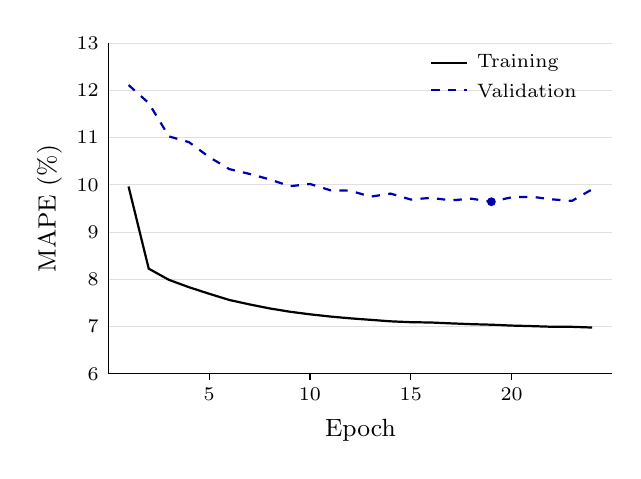
\begin{tikzpicture}[font=\small]
\draw[gray!25] (0,0.000) -- (6.400,0.000);
\node[left,font=\scriptsize] at (0,0.000) {6};
\draw[gray!25] (0,0.600) -- (6.400,0.600);
\node[left,font=\scriptsize] at (0,0.600) {7};
\draw[gray!25] (0,1.200) -- (6.400,1.200);
\node[left,font=\scriptsize] at (0,1.200) {8};
\draw[gray!25] (0,1.800) -- (6.400,1.800);
\node[left,font=\scriptsize] at (0,1.800) {9};
\draw[gray!25] (0,2.400) -- (6.400,2.400);
\node[left,font=\scriptsize] at (0,2.400) {10};
\draw[gray!25] (0,3.000) -- (6.400,3.000);
\node[left,font=\scriptsize] at (0,3.000) {11};
\draw[gray!25] (0,3.600) -- (6.400,3.600);
\node[left,font=\scriptsize] at (0,3.600) {12};
\draw[gray!25] (0,4.200) -- (6.400,4.200);
\node[left,font=\scriptsize] at (0,4.200) {13};
\draw (1.280,0) -- (1.280,-0.08);
\node[below,font=\scriptsize] at (1.280,-0.05) {5};
\draw (2.560,0) -- (2.560,-0.08);
\node[below,font=\scriptsize] at (2.560,-0.05) {10};
\draw (3.840,0) -- (3.840,-0.08);
\node[below,font=\scriptsize] at (3.840,-0.05) {15};
\draw (5.120,0) -- (5.120,-0.08);
\node[below,font=\scriptsize] at (5.120,-0.05) {20};
\draw (0,0) -- (6.400,0); \draw (0,0) -- (0,4.200);
\draw[thick, black] (0.256,2.379) -- (0.512,1.336) -- (0.768,1.194) -- (1.024,1.100) -- (1.280,1.017) -- (1.536,0.938) -- (1.792,0.882) -- (2.048,0.831) -- (2.304,0.789) -- (2.560,0.756) -- (2.816,0.728) -- (3.072,0.705) -- (3.328,0.686) -- (3.584,0.667) -- (3.840,0.656) -- (4.096,0.652) -- (4.352,0.641) -- (4.608,0.631) -- (4.864,0.624) -- (5.120,0.613) -- (5.376,0.606) -- (5.632,0.598) -- (5.888,0.597) -- (6.144,0.588);
\draw[thick, blue!70!black, dashed] (0.256,3.668) -- (0.512,3.439) -- (0.768,3.016) -- (1.024,2.942) -- (1.280,2.753) -- (1.536,2.600) -- (1.792,2.539) -- (2.048,2.470) -- (2.304,2.383) -- (2.560,2.411) -- (2.816,2.332) -- (3.072,2.326) -- (3.328,2.250) -- (3.584,2.289) -- (3.840,2.214) -- (4.096,2.235) -- (4.352,2.203) -- (4.608,2.225) -- (4.864,2.186) -- (5.120,2.242) -- (5.376,2.249) -- (5.632,2.216) -- (5.888,2.197) -- (6.144,2.344);
\fill[blue!70!black] (4.864,2.186) circle (1.6pt);
\node[below,font=\small] at (3.200,-0.45) {Epoch};
\node[rotate=90,font=\small] at (-0.75,2.100) {MAPE (\%)};
\draw[thick] (4.100,3.950) -- ++(0.45,0) node[right,font=\scriptsize] {Training};
\draw[thick, blue!70!black, dashed] (4.100,3.600) -- ++(0.45,0) node[right,font=\scriptsize,text=black] {Validation};
\end{tikzpicture}
\caption{Student-KD (best epoch 19).}\label{fig:curve-kd}
\end{subfigure}
